
\documentclass{acm_proc_article_sp}
\begin{document}
\title{Comunity Structure & Extremely Speculative Asset Dynamics}
%
\numberofauthors{6} 
\author{
\alignauthor
Nicolas Della Penna\titlenote{Dr.~Trovato insisted his name be first.}\\
       \affaddr{ANU}\\
%       \affaddr{1932 Wallamaloo Lane}\\
%       \affaddr{Wallamaloo, New Zealand}\\
%       \email{trovato@corporation.com}
% 2nd. author
\alignauthor
Eaman \titlenote{is first co-author.}\\
       \affaddr{MIT}\\
 %      \affaddr{P.O. Box 1212}\\
 %%      \email{webmaster@marysville-ohio.com}
% 3rd. author
\alignauthor Peter Kraft \titlenote{This author is the
one who did all the really hard work.}\\
       \affaddr{The Th{\o}rv{\"a}ld Group}\\
       \affaddr{1 Th{\o}rv{\"a}ld Circle}\\
       \affaddr{Hekla, Iceland}\\
       \email{larst@affiliation.org}
\and  % use '\and' if you need 'another row' of author names
% 4th. author
\alignauthor Lawrence P. Leipuner\\
       \affaddr{Brookhaven Laboratories}\\
       \affaddr{Brookhaven National Lab}\\
       \affaddr{P.O. Box 5000}\\
       \email{lleipuner@researchlabs.org}
% 5th. author
\alignauthor Sean Fogarty\\
       \affaddr{NASA Ames Research Center}\\
       \affaddr{Moffett Field}\\
       \affaddr{California 94035}\\
       \email{fogartys@amesres.org}
% 6th. author
\alignauthor Charles Palmer\\
       \affaddr{Palmer Research Laboratories}\\
       \affaddr{8600 Datapoint Drive}\\
       \affaddr{San Antonio, Texas 78229}\\
       \email{cpalmer@prl.com}
}
% There's nothing stopping you putting the seventh, eighth, etc.
% author on the opening page (as the 'third row') but we ask,
% for aesthetic reasons that you place these 'additional authors'
% in the \additional authors block, viz.
\date{today}
% Just remember to make sure that the TOTAL number of authors
% is the number that will appear on the first page PLUS the
% number that will appear in the \additionalauthors section.

\maketitle
\begin{abstract}


\end{abstract}

% A category with the (minimum) three required fields
%\category{H.4}{Information Systems Applications}{Miscellaneous}
%A category including the fourth, optional field follows...
%\category{D.2.8}{Software Engineering}{Metrics}[complexity measures, performance measures]

\terms{Theory}

\keywords{ACM proceedings, \LaTeX, text tagging} % NOT required for Proceedings


\section{Introduction}

Speculative bubbles are perceived to periodically take over markets \cite{garber2001famous}.
Going back at least to the \emph{South Sea} bubble in the early 18$^{\text{th}}$ century, well-informed parties  have invested knowingly in bubbles, and found it profitable \cite{temin2004riding}.
Today, the public notoriety of Bitcoin, together with its massive price increases and their associated publicity lead to an explosion of attempts to create ``the next Bitcoin''.
Collectively, these currencies are often referred to as ``cryptocurrencies'' or simply ``coins'', and a vibrant set of exchanges have emerged where these are traded, either for each other or money.
The majority of these coins have no possible future valuable in the long term, and their markets would appear to be driven largely by speculation.
Many of them appear to be nothing but attempts at turning a quick profit from inflating the implied valuation of a coin shortly after creating it.
This is driven by the extremely low cost and effort required to create a new coin, with most being minimal changes to parameters and branding of a pre-existing codebase.

Those who make and trade these coins communicate largely online, and much of their activity is concentrated on public forums. 
As such, price and volume data from these exchanges is freely available and widely aggregated\footnote{ these are however largely unregulated, often anonymous, and there is no way to account how much of reported volumes are manipulation attempts. The existence of attempts at arbitrage between them places some bounds on how blatantly the data can be manipulated for prices, but volumes are impossible to assess. },
%JULIAN: Whole footnote is one extra-long sentence!
and the source code to all of them being public is the norm%\footnote{cargo cult CS being derigour in the comunity}.
This makes cryptocoins
%JULIAN: cryptocoins is a new work--maybe avoid mixing the terms
an ideal lens through which to study the social life of a ``market mania'' \cite{cosma2008}.
Such a study is valuable both as a means of understanding the dynamics of bubbles themselves, but also from a computational social science perspective, to understand the ecosystem and lifecycles of these online communities.
%Such a study can serve in the computational social sciences a role analogous to that of lesion studies do in neuropsychology.
%JULIAN: Not obvious to me what the above analogy is without further explanation.


%\begin{figure}[h!]
%\end{figure}

We present a study of a large number of cryptocurrency ecosystems, 
using a novel dataset that combines measures derived from social networks of users in cryptocurrency forums, market data aggregated over dozens of exchanges, and properties of the software implementing the cryptocurrencies themselves.
From forums we identify the introducers of each coin and build measures of their position in the network based on
%which users have engaged with them
their patterns of engagement in forum threads
%threads in the forum
\emph{before} the coin is announced.
In this way we identify 376 coins that are announced by users of the forum and which can be mapped to price and volume data from exchanges.
Next, from price and transaction volume data we build measures of the subsequent activity that results from trading in the coin. 
We also assess if coins possibly embody technological innovation based on having more than trivial modifications to previously existing coins' source code.


%\begin{figure}
%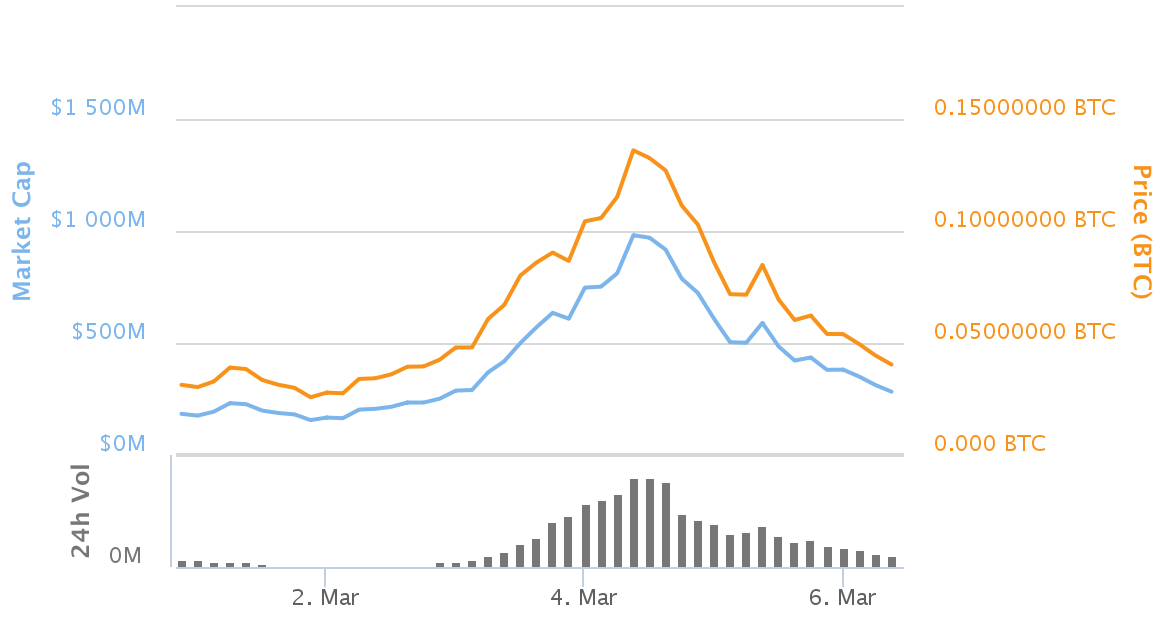
\includegraphics[width=\columnwidth]{AuroraCoin}
%\end{figure}

While the mechanisms that drive bubbles have been studied both theoretically 
\cite{abolafia1988enacting, earl2007decision, bakker2010social, harras2011grow}
and experimentally
\cite{moinas2013bubble},
% in the lab, 
an exhaustive dataset and study of the social networks of those promoting the asset has not been previously previously possible.
While the magnitude of the assets traded is certainly small relative to most financial and commodity markets, it is nevertheless much larger than
%JULIAN: Found this sentence a bit funny, not that I could improve upon it
even the most lavishly funded experimenter could hope for.
For example, the largest bubble in our dataset, AuroraCoin, reaches a valuation of one billion USD in March 2014,
with reported daily trading volumes of 6.8M USD, and sheds 90\% of its value in a week, and 99\% of its value in well under a year.
For context, this is equivalent to one quarter of Iceland's entire foreign exchange reserves in 2014,\footnote{4.1 Billon USD, The World Bank, Global Economic Monitor, accessed October 2015} the population of which AuroraCoin promoters claimed they would distribute half of the coins to.

\begin{figure}
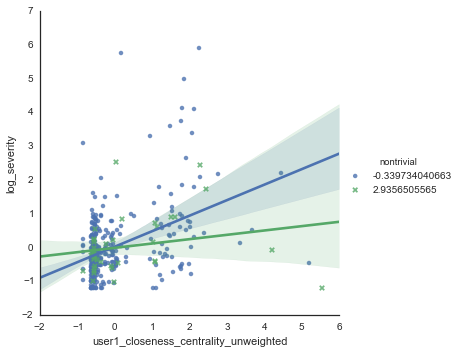
\includegraphics[width=\columnwidth]{severity_centrality}
\end{figure}

Using price and volume data we construct measures of both the magnitude and the severity of bubbles.
These are defined formally in our variable section,
%JULIAN: Give a section ref?
but their intuition is that we say the magnitude of a coin is large when a high volume in dollars of trades happens,
%JULIAN: Does it make a difference what it's measured in?
while we say a coin has a severe bubble if investing a fixed amount leads to loosing a large proportion. 
By considering the community structure that exists in the forum before a coin is introduced we are able to predict a substantial fraction of the variation in both the severity and magnitude of the resulting bubble.
This is a challenging task, and models that rely on either simple activity or network metrics metrics show almost no predictive out-of-sample power, unable to explain even 1\% of the variation in either task,
our best models perform an order of magnitude better in both tasks.
%JULIAN: R^2 of 0.1 (if I interpret correctly) doesn't sound impressive until you've argued the fundamental difficulty of the problem, you might wait to mention such numbers.
%JULIAN: Would sound more impressive if you just said "it performs an order of magnitude better"
The main driver of our explanatory power is the centrality of a user in the directed network derived from the forum. 
This effect appears to be mediated by whether a coin involves a nontrivial technological change, the direction of the interaction reversing depending on whether it relates to magnitude or severity.
%JULIAN: Above sentence is tough to parse, but kind of an important one.
Both the severity and the magnitude of bubbles increases with the centrality of the user who introduces the coins in the forums.  
Interestingly this effect is concentrated in different ways depending on whether the coin software is more than a trivial modification: trivial coins have more severe bubbles the more central their introducers are, while volume is greater the more central the introducer of a nontrivial coin is.




%JULIAN: Needs something outlining the paper's main results here, ideally a figure explaining the role of the various parts of the system.
%JULIAN: I'd tone down the footnotes

\begin{figure}
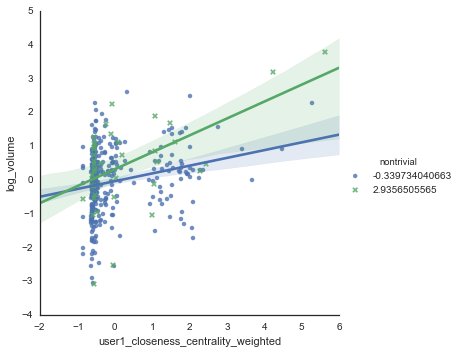
\includegraphics[width=\columnwidth]{volume_centrality}
\end{figure}

%Methodologically the free parameters in the way we do the weights on the weighted graph  is horrible, a million free parameters get introduced. follow up work for another paper: do some unsupervised feature learning over the dam forums threads to build the network; use some internal validity metric . Find political way of saying this in future work.
\section{Lit}

Agents structural strength within the discourse surrounding cryptographic currencies is particularly important, as these are almost entirely performative; the initial marketplace adoption of bitcoin is 
crash of  %87 http://www.iijournals.com/doi/abs/10.3905/jpm.1989.409242?journalCode=jpm 
“rapid rise of options” with the rise of the theory to price those options, in having currencies with zero entire costs
MacKenzie, Donald. "An Engine, Not a Camera."
While states can create the demand required for a currency system to run by compelling tax payment in it (for a recent example), non state sponsored currencies must find some other ways of creating demand.
The initial market for which bitcoin has been used (prices denominated in it, transactions only in it) where drug sales. citation.
New currencies have thus been floated with every single drug name possible. Many chains can claim to the same claim, so exchanges (since speculation is the only possible use of almost all of them) become de-facto stabilizers of who has a minimally viable claim. 









Network Diversity and Economic Development
http://www.sciencemag.org/content/328/5981/1029.full



"Hence, highly clustered, or insular, social ties are predicted to limit access to social and economic prospects from outside the social group, whereas heterogeneous social ties may generate these opportunities from a range of diverse contacts (1, 2)."

"Although both social and spatial network diversity scores were strongly correlated with IMD rank, we found a weaker positive correlation present using number of contacts and a negative correlation for communication volume."

"For example, whereas inhabitants of Stoke-on-Trent, one of the least prosperous regions in the UK, averaged a higher monthly call volume than the national average, they have one of the lowest diversity scores in the country. Similarly prosperous Stratford-upon-Avon has inhabitants with extremely diverse networks, despite no more communication than the national average. "




Predicting Spending Behavior Using Socio-mobile Features:
http://ieeexplore.ieee.org/xpl/login.jsp?tp=&arnumber=6693330&url=http%3A%2F%2Fieeexplore.ieee.org%2Fxpls%2Fabs_all.jsp%3Farnumber%3D6693330
free version:
https://scholar.google.com/citations?view_op=view_citation&hl=en&user=Ef1hJ8IAAAAJ&sortby=pubdate&citation_for_view=Ef1hJ8IAAAAJ:NaGl4SEjCO4C

Social behavior can be used to predict spending behavior in couples in regards to their prepensity to diversify the businesses they explore, become loyal customers and overspend. The results show that mobile phone social interaction patters can be more predictive than personality based features when predicting spending behavior. 

"We find that social behavior measured via face-to-face interaction, call, and SMS logs, can be used to predict the spending behavior for couples in terms of their propensity to explore diverse businesses, become loyal customers, and overspend"

"results show that mobile phone based social interaction patterns can provide more predictive power on spending behavior than personality based features. Interestingly, we find that more social couples also tend to overspend."




Money Walks: Implicit Mobility Behavior and Financial Well-Being:
http://journals.plos.org/plosone/article?id=10.1371/journal.pone.0136628

Spatiotemporal traits such as exploration, engagement and elasticity can be used to predict future finanical difficulties. 

"Hence, in this work we study a large-scale cross-sectional dataset of human spending across space and time, and connect it to the biological phenomena of “foraging,” a basic pattern of animal movement to gather foods and resources."

"we analyzed a corpus of hundreds of thousands of human economic transactions and found that financial outcomes for individuals are intricately linked with their spatiotemporal traits like exploration, engagement, and elasticity. Such features yield models that are 30\% to 49\% better at predicting future financial difficulties than the comparable demographic models."

"As shown in Fig 2, individuals with lower levels of education (High School, Middle School, or Primary School) were found to be more likely to be late for their payments and get into financial trouble. Users with higher age were marginally less likely to overspend, miss payments, or get into financial trouble. Last, male customers and married customers were less likely to miss their payments."

"The figure also shows that multiple mobility behavior features were statistically correlated with outcome variables, even after controlling for the effect of abovementioned demographic variables of age, gender, marital status, education, and work type."

"the behavioral features were found to be more significantly associated (in terms of p-values) and contain higher predictive power (in terms of odds ratios being further away from 1.0 in either direction) as compared to the demographic features."

"The evidence so far indicating that each of the spatio-temporal behavioral descriptors has significant association with different financial outcomes motivates their combination to predict the financial outcome"




Predicting personality using novel mobile phone-based metrics
http://dl.acm.org/citation.cfm?id=2456492
free version:
https://www.google.com/url?sa=t&rct=j&q=&esrc=s&source=web&cd=1&ved=0CCEQFjAAahUKEwivqbnj0L3IAhWIcT4KHZtqCOg&url=http%3A%2F%2Frealitycommons.media.mit.edu%2Fdownload.php%3Ffile%3DdeMontjoye2013predicting-citation.pdf&usg=AFQjCNGDDMiemMv9vPQGBd_NNP30sEr6MQ&sig2=CQk3pVIzJ3EmXlV0lD8oKA

"Using a set of novel psychology-informed indicators that can be computed from data available to all carriers, we were able to predict users’ personality with a mean accuracy across traits of 42% better than random, reaching up to 61% accuracy on a three-class problem."

"The goal of the present research is to show that users’ personalities can be reliably inferred from basic information accessible from all mobile phones and to all service providers."

"The model predicted whether phone users were low, average, or high in neuroticism, extraversion, conscientiousness, agreeableness, and openness with an accuracy of 54%, 61%, 51%, 51%, and 49%, respectively."



\section{Data Description}

We analize the 

\subsection{Prices, Exchanges, and Coin charactertistics}

Our main outcome measures are the severity of drop in the value of a unit of the asset, and the magnitude in USD of the transactions in them.
To obtain data for them we scrape three market aggregators 

We operationalize the intensity of a bubble as the proportion of a 1 dollar (TODO check currency base) that would be lost buying at the maximum price and selling after that proportionally to the volume of the market till the present, we call this severity.
We define the volume as the sum of the contemporaneous dollar (todo check) volume of trade.

As a secondary outcome measure we consider the number of exchanges that list the coin.


\subsection{Forum Discussions}

In order to study the effect of communication network around cryptocoins on
price variations, we collected all the posts from the most popular cryptocurrency
online community, bitcointalk.  Our data consisted of all the posts that were
made between January 2010 and July 2015 on the most active crypto-related forums:
\begin{enumerate}
  \item{Bitcoin Discussion:} This is the oldest forum on the website which mainly focuses
    on issues only related to Bitcoin. Interestingly, Satoshi Nakamoto, the alleged
    creator of Bitcoin made the first post on this forum in January 2010 and
    was active until January 2011. The presence of Satoshi in the data set enables us
    to study the position of various actors in the online community relative to Satoshi
    and its relation with the success or failure of cryptocoins they advocate or reject.

  \item{Altcoin Discussion:} This is the most active forum in the community
    with more than 730,000 posts as of July 2015, and dating back to June 2011.
    The discussions in this forum mainly evolve around alternative currencies
    other than Bitcoin. Users often discuss the merits or flaws of various
    altcoins or simply exchange technical information.
  
  \item{Announcement (Altcoin):} Community announcements such as development of 
    exchange client or addition of new features are made here. This is an important forum
    in our study as the creation of new altcoins are announced here. Whenever a new
    altcoin is announced to the community, the announcement is tagged with string ANN.
    This enables us to detect announcement of new coins into the market and identify
    the users who introduced them for the first time.

  \item{Mining (Altcoin):} Technical issues pertaining to mining (i.e. validating transactions)
    altcoins are discussed here.
  \item{Marketplace (Altcoin):} This forum contains the discussions on a wide-range of 
    market-related issues, such as price or volume trends, possible pump and dump schemes
    and exchange tips.

\end{enumerate}
TODO: CHECK AVERAGE NUMBER OF POSTS PER THREAD, and other statistics

Each forum consists of many subjects or threads initiated by different users.
Each thread contains several posts or replies, with an average of 10 posts per
thread.  The reply structure within each thread constitutes the basis of our
forum network, discussed below.  Each post has several fields which contain
valuable information in our context.
\begin{enumerate}
  \item{Subject:} Usually, the initiator of the thread chooses subject and all the
    following posts inherit the same subject.
  \item{Content:} The actual text of the message.
  \item{Position in the thread}: The later posts in the thread might not be as important
    as earlier posts and could be about issues other than the original topic of the thread.
  \item{Author}
  \item{Date}
\end{enumerate}

The community had only 10000 unique users until early 2013, however it grew considerably faster after 2013 and reached about 70000 by early 2015.
Nevertheless, there are only 10000 active users within any 30 day period on average.


\section{Forum Interaction Network}

Given the forum discussion data at the level of individual posts, we  construct a network capturing the structure of user discussions.
In this network, nodes are the forum users and directed edges represent 

% This paper did no such experimentation, maybe you did this alone and are welcome to put it in another paper.

%We experimented with different network construction methods, weight assignment schemes, and edge retention periods. For example, edges could be added based on co-appearance in each thread. 
%However, this approach quickly leads to a very dense network revealing little information about discussion dynamics.
%Moreover, the network could be unweighted or weights could be assigned to each edge based on a frequency of interactions between the two endpoints.
%Weights could also adjusted by size of the thread (i.e. an interaction in small threads counts
%more than an interaction in a large thread) and a decay factor (i.e. a recent interaction counts more than an old %interaction).
%Finally, the network could contain the interactions only within the past few days to capture short-term effect of information diffusion and influence dynamics.
%Alternatively, network construction could use all the interactions since the inception of the forums. The unlimited retention of interactions leads to a better view on long-term dynamics and more accurate identification of influential and senior users in the forum.


%In the following discussion, we only include the results from directed unlimited network.
The network is directed since the \textit{edges point from posters within each thread to thread-initiators}. The omission
of co-appearance edges leads to a sparser network which isolates the communication
patterns around ``dialogue-shapers''. The network is unlimited since all such interactions
from the inception of bitcointalk are included in its construction. The longer timespan
of interactions captures relevant information on seniority and community influence 
which are obtained through long-term and persistent presence in the forums.
We edges on this network are weighted by the number of times a poster replies
to a thread-initiator in unique threads. We chose the unlimited directed network
since it proved to be the most informative and simplest to interpret.

Prior to construction of the network, we merged posts from all forums into a
single large large forum since the community base of all five forums mentioned
above is made of the same users and we are mostly concerned about influence and
aggregate information flow among users, rather than the exact topic of the discussion.
The network construction involves replaying the posts over time sorted by their date and updating the
discussion graph accordingly. Whenever a new altcoin was introduced
in the forum for the first time, the user who introduced it and a snapshot of the graph was taken.
The position of the first introducer in the network snapshot and its general structure 
will be used for extracting various network measures corresponding to that coin. Our analysis
uses these per-coin for evaluating the performance of each coin.


In order to avoid confounding between a coins price moves and the attention this mkes the comunity in the forums pay to discusions of the coin , we analyze the discussion network up to the time of coin introduction to the community.
%TODO Do we use the date of the ANN or the date of the first trade?!?! NIKETE & EAMAN.
%The identification of true introductions of new altcoins is a difficult process prone to many false-positives. 
The  majority of such introductions are made in the \textit{Announcement} forum and are preceded with the ``ANN'' tag.
%Our identification strategy <- this has a specific technical meaning in econ
We look for the first mention of both the coin symbol \textbf{and} its descriptive name in the subject of a thread which contains the announcement tag. 

The first mentions of either the coin symbol \textbf{or} the its name are used fall-back in case the more restrictive \textbf{and} requirement did not detect the coin. 
Using this identification strategy, we were able to detect the first introduction of 554 altcoins out of 679.
The forum user who initiated such a thread is assigned as the  introducer of the coin to the community.
%TODO: add validation results table wrt mapofcoins data here

\section{Results}


\begin{figure}[h]
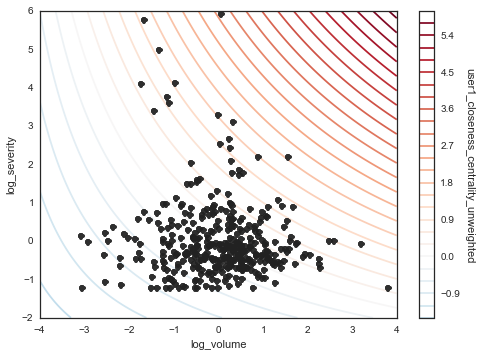
\includegraphics[width=\columnwidth]{centrality_volume_severity}
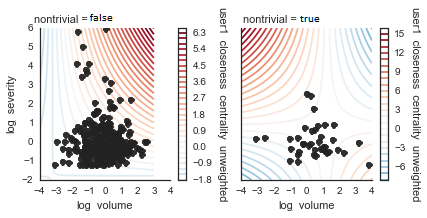
\includegraphics[width=\columnwidth]{centrality_volume_severity_nontrivial}
\end{figure}

\section{Conclusion}


The total variance accounted for is small, so you need a discussion like "results suggest that bubble dynamics may be strongly influenced by a core set of participants, but that traditional network measures on the aggregate discussion graph do not provide a tight characterization of this core group.  We are looking at coarse (positive/negative, detailed/cursory) semantic analysis of the discussion, and evidence of prior cooperation between pairs of participants in other altcoin markets, in order to attempt this more accurate characterization of core participants and their actions.



\section{Data}



\section{}



\section{Acknowledgments}

%
% The following two commands are all you need in the
% initial runs of your .tex file to
% produce the bibliography for the citations in your paper.
\bibliographystyle{abbrv}
\bibliography{sigproc}  % sigproc.bib is the name of the Bibliography in this case
% You must have a proper ".bib" file
%  and remember to run:
% latex bibtex latex latex
% to resolve all references
%
% ACM needs 'a single self-contained file'!
%
%APPENDICES are optional
%\balancecolumns
\appendix
%Appendix A
\section{Headings in Appendices}
The rules about hierarchical headings discussed
\balancecolumns
% That's all folks!
\end{document}
